\documentclass{article}
\usepackage{mathtools,natbib}

\author{Michael Hay, Department of Earth and Space Sciences}


\begin{document}

\title{Ph.D. proposal: Mesoscale stratigraphic disturbances in ice sheets relating to plastic anisotropy}
\maketitle
\section{Introduction}
Ice cores from ice sheets provide an important record of past climate.  For accurate interpretation, a ice depth-age relationship is needed. The ice-sheet stratigraphic record is an important tool in constructing this relationship. However, ice-sheet stratigraphy can be disturbed, which can make paleoclimate interpretation difficult. Layers can be overturned, resulting in older ice lying above younger ice. As well, boudinage can occur, potentially removing layers from an ice core record. Especially on the meter or smaller scale, it is likely that a large portion of stratigraphic disruptions are due to the plastic anisotropy of ice.

Individual ice crystals have strong plastic anisotropy, deforming most easily in shear in the basal plane orthogonal to the crystallographic c-axis. Other orientations are around 100 times harder. This can lead to disturbances in several different ways. In both simple shear and vertical uniaxial compression, c-axes tend to cluster near vertical. Vertical maximum fabrics are soft under horizontal simple shear, because the basal planes are aligned with the imposed shear stress. If there is an initial open wrinkle in the stratigraphy, the enhanced simple shear can lead it to overturn into a recumbent fold \citep{throstur2002}. Boudinage can occur if there is a harder layer (under extension) surrounded by softer layers. This has likely been observed in electrical conductivity measurements at the WAIS divide core. \citet{alley97} as well found ``stripes'' of non-vertical grains in otherwise vertical-maximum fabric. Similarly, ``tilted cone`` fabrics can occur, where the maximum of the orientation distribution function is off-vertical \citep{throstur2002}. Such fabrics can lead to strain in different components than the applied deviatoric stress. This is a likely mechanism to produce smaller-scale stratigraphic disturbances, even outside of the influence of the bed. Previous work on anisotropic ice flow modeling, such as \citet{gillet2005}, has not allowed for general anisotropic viscosity. In addition, it is likely that the coupling of anisotropic flow and fabric evolution is dynamically unstable. For example, under simple shear, fabrics softer under simple shear will evolve towards a softer single maximum faster than initially harder-oriented grains. This can enhance small initial variations in fabric, and induce the formation of shear bands. In addition, \citet{montgomery-smith2011} analytically found that 3-dimensional Stokes flow of a fluid with dense rigid-fiber inclusions, whose orientation distribution function determined by Jeffery's equations, is unstable. This is mathematically very similar to ice flow coupled to Jeffery's equation, with the ice only deforming by basal glide, except that the ice posesses nonlinear viscosity.

\section{Current work}
Studying anisotropic ice flow requires a coupled approach between fabric evolution and anisotropic flow. To this end, I have developed an strain-induced ice-fabric evolution model which incorporates a variety of physical processes. We are currently preparing a manuscript based on this model. It treats the fabric as a finite collection of grains, each with properties such as radius, dislocation density, and connectivity between different grains. Unlike previous fabric evolution models, this is mass conservative. Grains exchange mass through their nearest neighbors, thus grains can only grow at the expense of others. Dynamic recrystallization is treated as probabilistic, with the probability depending on temperature and accumulated dislocation density. This is justified because there are unobserved properties which control recrystallization at the small scale, such as inclusions and subgrain-scale dislocation density variability.

I have forced the model with thin section data from the West Antarctice Ice Sheet (WAIS) divide ice core. Ensemble runs using bootstrapped data show that fabrics which have statistically the same distribution do not converge over time. The strengths of individual fabric realizations can oscillate with respect to other samples. This is seen in the figure using earth mover's distance as a measure of distribution distance from a perfect girdle. This occurs even if there is no recrystallization, and is likely due to the effects of fabric connectivity. These differences are related to sample size. However, several hundred grains can occupy a large volume. Despite two samples being taken from the same distribution, the response to applied stress can nonetheless vary greatly. Thus, fabric variability could be an important driver behind flow disturbances. 

\section{Research plan}
In the very short term, we will submit our manuscript regarding the fabric model. Subsequently, we will work on a coupled anisotropic flow model with a continuum fabric evolution model to look at meter-scale flow. The fabric evolution portion will use a tensor-closure approximation of the fabric in a Jeffery's-type equation \citep{jeffery1922} together with a continuum analogue of the discrete nearest neighbor interaction from \citet{throstur2002}.

The flow component will be standard power-law Stokes flow, but with an anisotropic viscosity tensor represented by a $6 \times 6$ Voigt matrix generated from the fabric distribution. The strain-rate dependent factor of viscosity is assumed to be scalar. For a numerical scheme, we will likely use a simple finite-difference approach, with the fabric evolution component using an upwind method. While there is some coding difficulting inherent in it being a 3D model, the anisotropic viscosity is not difficult. I have already done much of the work in computing viscosity. The model will also use a simple cubic geometry, with horizontal periodic boundary conditions.

This will allow us to look at numerous issues regarding anisotropic flow. Boudinage and recumbent folding from initial folds can be investigated. In addition, we will be able to test how spatial variability in ice fabric affects stratigraphy. In particular, we will see if spatial differences in fabric persist over time. We will also test whether fabric variations can produce vertical strain under horizontal simple shear. In addition, we will see if the coupled numerical model exhibits the instabilities suggested by \citet{montgomery-smith2011}. This work will shed light on what conditions flow disturbances can happen, and over what length scales they can disturb stratigraphy. That will allow for more accurate knowledge of the errors expected in depth age relationships, and may allow for better dating of ice in regions of disturbed stratigraphy. The coupled finite difference model is expected to take roughly a year.

As an aside to the numerical model, we may also adapt the work of \citet{montgomery-smith2011} for ice with nonlinear viscosity. It is very likely that the same instabilities occur, but the nonlinearity of viscosity may enhance the dynamic instabilities.

\begin{figure*}
\caption{90\% confidence interval and median of evolution of the distribution of the fabric sample at the top of the core, inferred from repeated bootstrap samples of the thin section data. Two sample realizations are also included.}
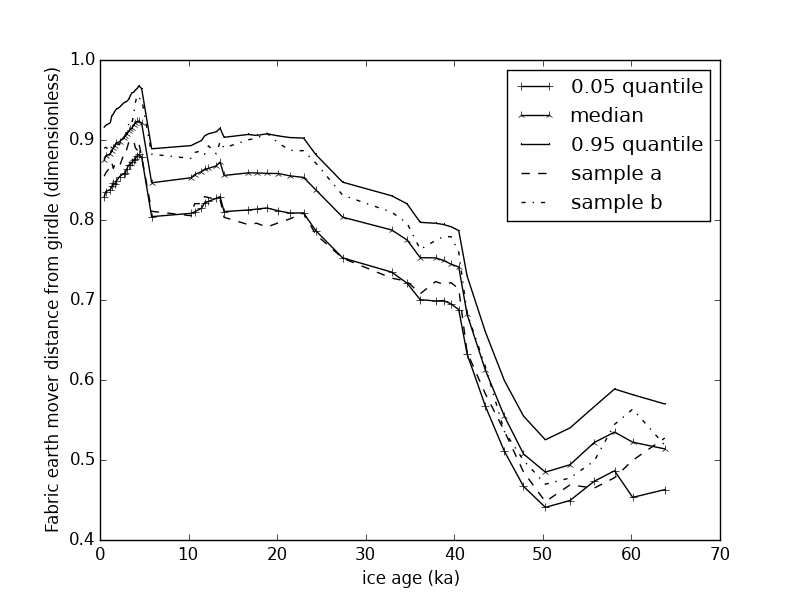
\includegraphics[width=12cm]{ci}
\end{figure*}


\subsection{Funding}
This research is currently funded by NSF Grant 0636996 for the study of anisotropic ice flow. This will continue until June 2016, although an extension is likely. If funding is needed beyond then, we will seek another grant or rely on TA funding. 

\bibliographystyle{agu}
\bibliography{anis}

\end{document}
